
%%%%%%%%%%%%%%%%%%%%%%% file typeinst.tex %%%%%%%%%%%%%%%%%%%%%%%%%
%
% This is the LaTeX source for the instructions to authors using
% the LaTeX document class 'llncs.cls' for contributions to
% the Lecture Notes in Computer Sciences series.
% http://www.springer.com/lncs       Springer Heidelberg 2006/05/04
%
% It may be used as a template for your own input - copy it
% to a new file with a new name and use it as the basis
% for your article.
%
% NB: the document class 'llncs' has its own and detailed documentation, see
% ftp://ftp.springer.de/data/pubftp/pub/tex/latex/llncs/latex2e/llncsdoc.pdf
%
%%%%%%%%%%%%%%%%%%%%%%%%%%%%%%%%%%%%%%%%%%%%%%%%%%%%%%%%%%%%%%%%%%%


\documentclass[runningheads,a4paper]{llncs}

\usepackage{amssymb}
\setcounter{tocdepth}{3}
\usepackage{graphicx}

\usepackage{url}
\urldef{\mailsa}\path|{caldwelt, david.t.coleman, nikolaus.correll}@colorado.edu|    
\newcommand{\keywords}[1]{\par\addvspace\baselineskip
\noindent\keywordname\enspace\ignorespaces#1}

\usepackage{color}
\usepackage{wrapfig}


\begin{document}

\mainmatter  % start of an individual contribution

% first the title is needed
\title{Robotic Manipulation for Identification of Flexible Objects}

% a short form should be given in case it is too long for the running head
\titlerunning{Robotic Manipulation for Identification of Flexible Objects}


\author{T. M. Caldwell and  D. Coleman and N. Correll%
\thanks{
This work was supported by a NASA
Early Career Faculty fellowship NNX12AQ47GS02. We are grateful for this support.}%
}
%
\authorrunning{Robotic Manipulation for Identification of Flexible Objects}
% (feature abused for this document to repeat the title also on left hand pages)

% the affiliations are given next; don't give your e-mail address
% unless you accept that it will be published
\institute{Department of Computer Science, University of Colorado,\\
1111 Engineering Dr, Boulder, CO 80309, USA\\
\mailsa}

\toctitle{Lecture Notes in Computer Science}
\tocauthor{Authors' Instructions}
\maketitle

\begin{abstract}
This paper provides preliminary insight into stiffness profile identification of a complex flexible object by robotic manipulation. The object is in the shape of the letter `Y', chosen to resemble a living plant.  The object is approximately modelled as a spring mass system. The robot manipulates the object with one or two arms grasped at the ends of the `Y', and makes visual measurements which locates the object's position in space.  Identification results from an optimization approach are compared for both one and two arm manipulation and sensing with and without vision. The results are not consistent with the expected physical object's properties due to a failure to observe the motion dependence between the object's connected segments. The result provides insight into the problem of assessing the minimal information needed to identify the stiffness of a flexible object, an issue of importance to automated approaches.% Another explanation is a segment's motion is insufficient to be observed due to the motion of other segments dominating the sensor's location's motion.
\end{abstract}

\section{Introduction}

\begin{figure}[!htb]
\centering
\def\svgwidth{.95\textwidth}%500pt}
\input{baxter_y.pdf_tex}
\caption{The physical experiment, vision capture (in green), and simulation of baxter manipulating a flexible object.} %The vision capture is shown in MoveIt! and the simulation is done in \texttt{trep}.}
\label{fig-baxter_y}
\end{figure}

The goal of this work is to use a robotic arm and an external vision system to identify the behavior of the flexible object shown in Figure \ref{fig-baxter_y}. This is an important step toward manipulation of flexible objects such as living plants, rubber tubes, and clothes \cite{wakamatsu2006knotting,saha2007manipulation,bell2010flexible,jimenez2012survey}.  

There are many methods to model and simulate flexible objects \cite{khalil_payeur,lang_etal}.  A common approach is to model the object as a lattice or collection of links of masses and springs \cite{sahari_etal,wakamatsu_etal,khalil_payeur}.  This approach has been used to simulate linear object like strings, hair, and electrical cables for which the model is a series of masses linked together with springs. %%% MISSING: LIMITATIONS OF THIS APPROACH  

% 3. What are you doing that is new and why do you think it will be successful
We also model the flexible object as a spring mass system.  In \cite{caldwell_coleman_correll_iros} we modeled a rubber tyre in such a way, and identified the spring constants for its uniform stiffness with a novel identification method. In this paper, we explore a more complex structure in the form of a foam `Y' made of tubes with differing stiffnesses. We observe that not only must we carefully plan where to manipulate an object in order to sufficiently excite all of its degrees of freedom for measurement---in this case at the end of each Y---but that this is insufficient to accurately identify its stiffness profile, even with additional measurements made by an external vision system. The failure in identification is due to the motion dependence between the object's segments.

Two types of sensing are investigated. The first is the joint angles and torques of Rethink Robotic's Baxter robot's arms. The second is an external vision system that produces a point cloud of the object and through filtering and fitting, can locate specific points on the object. We note that the vision cannot make any torque or force measurements and as such can not directly measure stiffness properties.

%Even with measurements at distinct locations on the object, such as the junction point of the `Y' object and each of its extremities with two arms, or with additional sensors such as a camera that is used to localize the object in the first place. In particular we note that it is not possible to automatically generate these grasp points unless the boundaries between sections with different stiffness are known. 

%We then show how vision allows us to find a stiffness profile that is more in accordance with physical reality, and show that we are able to accurately predict the motion of the structure using these values when compared with data from the camera

%The identification approach is taken from the our work in \cite{caldwell_coleman_correll_iros}. In that paper, we identified the spring constants of a flexible loop using touch alone where the only measurements were the joint torques and angles of a robotic arm. %In the current paper, we extend this result to also use visual perception during the identification. Furthermore, the object under consideration in this paper has a more complex geometry.  We find that identification from touch using a single robotic arm is not sufficient and as such we need additional measurements like vision.  The new object is shaped similar to the letter `Y' and was chosen in part due to its resemblance to plant life.  To the best of our knowledge, no one has used a robot to identify parameters of a flexible object with such a geometry, nor has anyone planned robotic manipulation of such a flexible object.

%In order to identity parameters of the object, such as its stiffness profile, we assume the robot has rigidly grasped the object at one of or both of the object's ends with one or two of its arms. The robot then bends, twists, and stretches the object. During the manipulation, the robot measures the arm's joint torques and joint angles.  Furthermore, a vision system captures the movement of the full object in three dimensions.  With this information, it is possible to back out mechanical properties of the loop in order to generate an accurate model for future control and manipulation. 

We model the object with the same underlying mechanics as the robot arm---i.e., as a collection of rigid bodies connected at joints by springs---allowing us to utilize the vast theory of rigid body mechanics \cite{murray_li_sastry}. Also, this enables planning and control to be done in the combined arm and object configuration space instead of only the end effector space or object space.  We then use an optimal control approach in \cite{caldwell_coleman_correll_iros} for calculating model properties that best match the behavior of the flexible object. The physical experiment, the vision capture, and the model can be viewed in Figure \ref{fig-baxter_y}.

As in \cite{caldwell_coleman_correll_iros}, we use variational integrators to simulate the robot and object.  Variational integrators can be used to describe discrete-time equations of motion of a mechanical system.  They are designed from the least action principle and have good properties that agree with known physical phenomenon like stable energy behavior \cite{pekarek_murphey}. All simulations were implemented in \texttt{trep} \cite{johnson_murphey_scalable,johnson_murphey_linearization}, which is a tool to simulate articulated rigid bodies using midpoint variational integrators.

%Finally, we demonstrate how to use optimal controls to plan a trajectory---i.e. calculate configurations and controls---that maneuvers the object from one configuration to another. Furthermore, we use this result along with a feedback loop to plan a trajectory that moves a point on the flexible object near a desired location in space.

\subsection{Organization of this paper}
This paper is organized as follows: Section \ref{sec-exp} sets up the experiment with the robot and flexible object. In Section \ref{sec-sim}, the flexible object is modeled as a connection of springs and masses. This section also reviews variational integrators. Section \ref{sec-vis} discusses the visual perception system and the techniques to filter and model fit the measured data. Section \ref{sec-id} reviews the identification algorithm from \cite{caldwell_coleman_correll_iros}. Section \ref{sec-id_eg} conducts the identification on the flexible object and compares identification with and without vision, as well as discusses the results..% Finally, Section \ref{sec-plan} provides the details on applying optimal control for planning a trajectory for the flexible object.

\section{Example Experiment Setup}
\label{sec-exp}
\begin{figure}[!htb]
\centering
\def\svgwidth{.6\textwidth}%500pt}
\input{baxter_y_sim.pdf_tex}
\caption{Model of Baxter manipulating a flexible object. The object is composed of 3 tubes, each approximated with four rigid links. The spheres illustrate the location of the masses and their relative values. The tube segments are labelled $T_1$, $T_2$, and $T_3$, and the points at the ends of the tube are $w^{T_1}$, $w^{T_2}$. and $w^{T_3}$.}
\label{fig-baxter_y_sim}
\end{figure}

The goal of the example experiment is to identify stiffness properties of a flexible object. The flexible object has the shape of the letter `Y'.  It was chosen to resemble the basic geometry of a living plant. The base, or `trunk' is attached to the ground and is labelled $T_1$. We investigate two scenarios. In the first, the robot has the point $w^{T_2}$ of branch $T_2$ grasped, and the branch $T_3$ is free (refer to Figure \ref{fig-baxter_y_sim}).  In the second scenario, the robot has both points $w^{T_2}$ and $w^{T_3}$ grasped using both arms. The goal is to manipulate the grasped branch so that the movement of the uncontrolled free branch can be predicted. %Due to the flexibility of the object it is not immediately clear how to do this planning.
% a manipulation that moves the free branch to the desired region. 

To improve prediction, we conduct the parameter identification optimization algorithm in \cite{caldwell_coleman_correll_iros} in order to identify the model's stiffness properties. The identification is made with physical contact data---i.e. joint angle and torques from one or two arms---and a vision system to capture the motion of the full flexible object. The identification process is the same as in \cite{caldwell_coleman_correll_iros} once the vision data has been fitted to the model. % Finally, we use the optimal control technique from \cite{hauser} to calculate a trajectory to move the flexible object from one configuration to another.

The flexible object is foam tubing with differing widths for each of the $T_1$, $T_2$, and $T_3$ sections. The three tubes are connected with a `Y' PVC joint and glue.  The trunk tube has length 0.813m and mass 0.064Kg. It is the widest tube with radius 0.032m. The grasped tube has length 0.610m and mass 0.015Kg and is the second widest tube with radius 0.025m. The free tube has length 0.737m and mass 0.016Kg. It is the thinnest with radius 0.019m.  %The tube widths are mentioned because we expect the relative twisting stiffnesses of each tube to correlate with their widths. 

We use Rethink Robotics' Baxter robot \cite{guizzo2011rethink} to both manipulate and measure the object.  Baxter's arms each have 7 degrees of freedom.  The arms are designed for compliance by means of series elastic actuators in each joint that allows for force sensing and control.  Baxter publishes the joint angles and torques at 100Hz.  A picture of Baxter manipulating the flexible object is in Figure \ref{fig-baxter_y}. 

\section{Model and Simulation \label{sec-sim}}
\label{sec-sim}
We model the flexible object as a spring mass system by approximating the $T_1$, $T_2$, and $T_3$ segments each with four rigid links of uniform lengths and masses, connected by joints with torsional springs---see Figure \ref{fig-baxter_y_sim}. Each joint is 3-dimensional allowing for bending and twisting motions of the flexible object. In total, the flexible object is 36 dimensional. The goal of the identification, Section \ref{sec-id}, is to identify the torsional springs' spring constants. We label these parameters as $\rho$.

Due to Baxter's 7 degrees of freedom arms, the system of Baxter grasping one end of the flexible object (neglecting the other arm) has a total number of 43 configuration variables. When grasping both ends of the object, (using both arms) the model has a total number of 50 configuration variables. The dimensions, inertia, and other information concerning Baxter's arm can be obtained at \url{https://github.com/RethinkRobotics}.  

\subsection{Simulation}
The model for both Baxter's arm and the flexible object are a series of rigid links connected by rotational joints. As such, the dynamics of both the manipulator and the object can be handled together. We use \emph{variational integrators} to simulate the system dynamics.   Variational integrators are a discrete-time representation of the equations of motion of a mechanical system.  They are designed from the least action principle and have good properties that agree with known physical phenomenon like stable energy behavior \cite{pekarek_murphey}.  

Simulations are for a finite time interval $[0,t_f]$ with discrete times $t_0,t_1,\ldots,t_{k_f}$, where $t_0 = 0$, $t_{k_f} = t_f$ and $k_f+1$ is the total number of discrete times in the interval. The simulation---i.e. the solving of the system dynamics---will result in a state $x_k:=x(t_k)$ for each $k$.  For variational integrators, the state is composed of the configuration, labelled $q_k$ for time $t_k$, as well as a term labelled $p_k$, also for time $t_k$. For systems without external forcing, $p_k$ is the conserved momentum.  For the purposes of this paper, it can simply be thought of as analogous to the discrete velocity, which is often paired with $q_k$ to make up the state.  The state is $x_k:=[q_k,p_k]^T$. 

The literature on variational integrators \cite{marsden_west} provides a one-step mapping to update the state at the previous time $x_k$ to the next time $x_{k+1}$.  We provide a short high-level review of variational integrators.  We write the one-step mapping which constitutes the systems equations of motion as 
\begin{equation}
x_{k+1} = f(x_k,\rho,t_k).
\label{eq-fk}
\end{equation}
Here, $f$ explicitly depends on the previous state, time, and the parameters which we wish to identify.  While we write the equations of motion as an explicit equation, the equations are in fact implicit and rely on root solving to update the state. 

The equations encapsulate the system's Lagrangian, any external forcing, holonomic constraints, as well as a choice of quadrature for approximating integrals.  The function $f$ can be linearized. We write 
\begin{equation}
A_k = \frac{\partial}{\partial x_k}f(x_k,\rho,t_k) \textrm{ and } B_k = \frac{\partial}{\partial \rho}f(x_k,\rho,t_k).
\label{eq-lin_fk}
\end{equation}
The equations to calculate the linearization with respect to the state and parameters can be found in \cite{caldwell_coleman_correll_iros}. They are needed for calculating the gradient for parameter identification as part of an iterative optimization.

\subsection{Simulation of Example}
We use variational integrators to simulate Baxter manipulating the flexible object through the simulation tool \texttt{trep} \cite{johnson_murphey_scalable}.  The tool simulates articulated rigid bodies using midpoint variational integrators.  It additionally provides partial derivative calculations that we need for the system linearization, Eq.(\ref{eq-lin_fk}). 

The system of Baxter manipulating the flexible object with a single arm has a 43 dimensional configuration. Therefore, the system's state,  $x_k = [q_k,p_k]^T$, is 86 dimensional. For the system of Baxter manipulating with both arms, the configuration is 50 dimensional and the state is 100 dimensional. The discrete dynamics $f$, Eq.(\ref{eq-fk}), is given by the discrete system Lagrangian, discrete external forcing, and holonomoic constraints---see \cite{caldwell_coleman_correll_iros,marsden_west}.  The system Lagrangian is specified by the kinetic and potential energies of Baxter and the object.  External forces enter the system through the torques applied by the motors at each of Baxter's joints.  Additionally, holonomic constraints are needed to ensure that Baxter's end effectors remain in contact with the object.  We chose a time step of $0.01$ seconds, which matches the broadcast frequency of Baxter. 

Nominally, the simulation will perfectly agree with Baxter's measured joint torque and angles for a given experiment. However, due to model and sensor disturbances, which are always an issue for real systems, this will not be the case. Furthermore, since the system is unstable---i.e. small disturbances can result in large changes to trajectory---directly feeding the measured torques into the model will not result in a meaningful simulation. Therefore, the measured joint torques, labelled $\overline{F}$, and measured joint angles, labelled $\overline{b}$, must be filtered through a feedback loop. We use a simple proportional control law with gain $K$: 
\[
F_k = \overline{F}_k - K_k (b_k - \overline{b}_k),
\]
where $F$ and $b$ are the simulated joint torques and angles for the filtered control input.  When $K$ is large, the effect the parameters have on the simulation is dominated by the control and as such, the system cannot be identified. However, if $K$ is too small, the system will remain unstable and not track the measured trajectory well enough to be meaningful.  Correctly choosing $K$ for the purposes of parameter identification of unstable systems is left for future work.  For this paper, we chose $K$ from a finite horizon LQR which results in an optimal feedback gain from the model linearized around $b_{meas}$ and a quadratic cost functional (see \cite{anderson_moore} for LQR).  The tradeoff between tracking the joint angles or joint torques is directly represented in the quadratic cost for specifying the size of $K$.


\section{Vision}
\label{sec-vis}
%For verification and improvement of the parameter identification algorithms, t
With the goal to improve parameter identification, the flexible object is visually tracked using an out of the box depth sensor, the Asus Xtion Pro Live. The depth sensor captures a point cloud, $G$, of the experiment. Processing $G$ consists of three steps: filtering, segmentation, and graph creation. 

A filtering component within the motion planning framework MoveIt! \cite{coleman_etal_barrier} performs the first step of self-filtering. It removes points detected on the robot’s body and arms. This is accomplished using the realtime joint states and calculated coordinate transforms to determine the robot’s configuration within the point cloud. A small amount of padding is included in the filtering to account for calibration error. The Point Cloud Library (PCL) \cite{rusu20113d} provides the second level of filtering, removing points detected behind the robot and on the floor. Finally, a statistical outlier removal filter removes remaining noise and measurement errors.

The segmentation of the filtered point cloud $G_{filtered}$ is accomplished using a custom algorithm built on top of PCL. This step converts the $T_1$, $T_2$, and $T_3$ sections (refer to Figure \ref{fig-baxter_y_sim}) of the object into segmented components that can later be turned into a graph, as shown in Figure \ref{fig-vision}. The lowest point in the point cloud (aligned with gravity) seeds  the algorithm. The $k_1$ nearest neighbors to this point is then chosen using a Kd Tree to represent a “segment” $s$ of the plant model. The centroid of $s$ is calculated and a second $k_1$ nearest neighbors search finds a centered segment $s_{centered}$ at the base of the plant.

\begin{figure}[!htb]
\centering
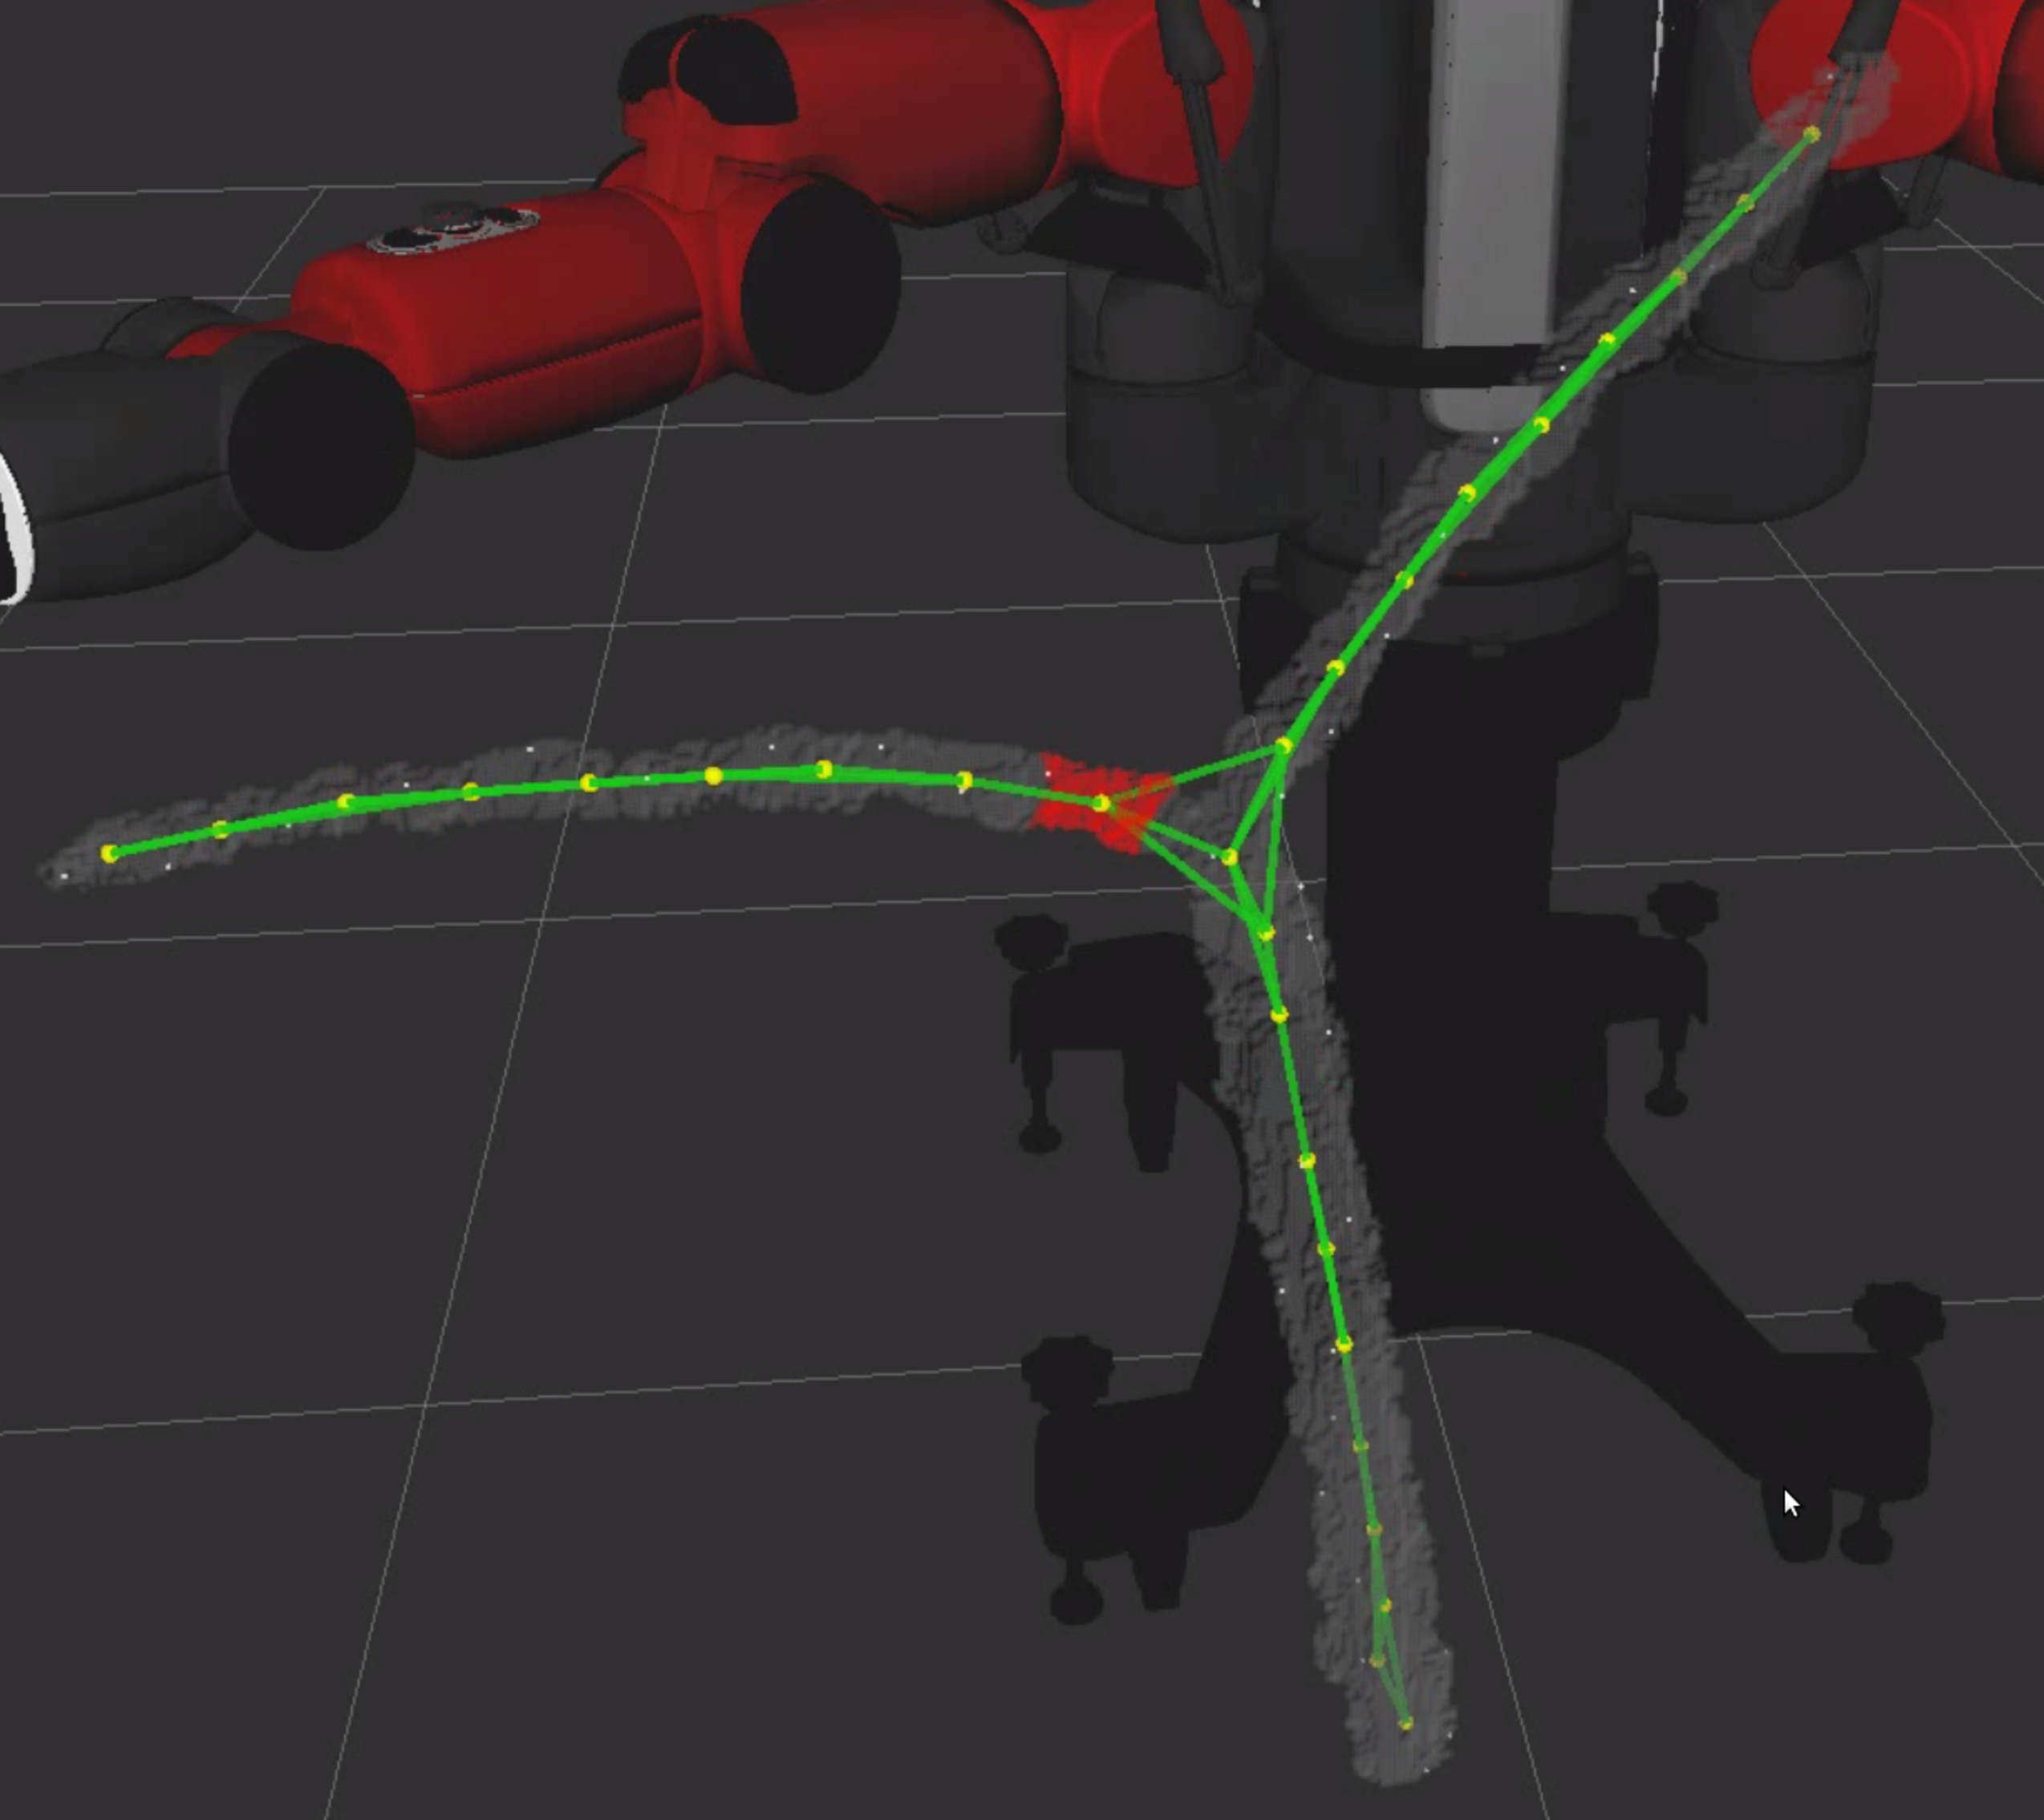
\includegraphics[width = 220pt]{vision_component}
\caption{Vision of flexible object.}
\label{fig-vision}
\end{figure}

Assuming the number of points in $s_{centered}$ are above a minimum threshold (to remove noise), the 3d centroid of $s_{centered}$ is added to a processed graph $G_{processed}$ and the points in $s_{centered}$ are removed from $G_{filtered}$. The next nearest neighbor to $s_{centered}$ is chosen as the new segment starting point and the algorithm repeats. Occasionally, there are insufficient nearest neighbors in a segment if, for example, the algorithm has reached the end of a plant branch. In this case, a random point is chosen in the remaining point cloud $G_{filtered}$ to continue the search, until no further points remain.

The final processing step takes the disconnected points in $G_{processed}$ and performs one final series of nearest neighbor searches to connect the nodes together to represent a flexible object modeled as a series of connected rigid bodies. These connected rigid bodies give a surprisingly accurate three dimensional reconstruction of a flexible object in soft-realtime, processing new point clouds at a rate averaging 3 hz. %Figure \ref{fig-vision} shows a single frame of processed vision data $G_{processed}$.


\subsection{Fitting to Model \label{sec-fit}}

The processed points in $G_{processed}$ need to be fitted to the static model of the plant to be useful. The model is a discretization of the physical object where the flexible object's configuration specifies the location of the discretization points. Label the object’s configuration as $q_o$. 

The fitting is a calculation on $q_o$ and is accomplished as follows: Let $G_{model}(q_o)$ be a graph specified for configuration $q_o$ with the discrete points as its vertices and adjacent points in the model as its edges. Any two adjacent points in $G_{model}(q_o)$ can be connected by a line segment in space. Let $L_{model}(q_o)$ be the collection of these line segments. Further, let $d(p,\ell)$ be the shortest Euclidean distance between the point $p\in G_{processed}$ and line segment $\ell \in L_{model}(q_o)$. Define $d(p,L_{model}(q_o)) := \min_{\ell\in L_{model}(q_o)} d(p,\ell)$ as the least distance between $p$ and any line segment in $L_{model}(q_o)$. This can be done for each $p\in G_{processed}$. The fitting is given by the $q_o$ for which the points in $G_{processed}$ are nearest the line segments $L_{model}(q_o)$---i.e. by the optimization program
\begin{equation}
\arg \min_{q_0} \sum_{p\in G_{processed}} d(p,L_{model}(q_o)).
\label{eq-fit_prog}
\end{equation}

\subsection{Vision Tracking Concerns \label{sec-vis_disc}}

A number of tuned parameters make the vision filtering and fitting algorithms sensitive to object size, the distance between the camera and object, and variability of the object's thicknesses. However, it works well for our experimental goals.

One major shortcoming of the vision tracking pipeline developed for this experiment is occasional loss of data due to buffering issues and self occlusion. Because of the computational complexity of our flexible object manipulation pipeline, the experiment was run on 3 distributed commodity PCs using ROS \cite{quigley2009ros}. A common issue is clock time synchronization between the three PCs, and ROS messages being dropped due to full buffers. This causes the robot transforms to be published with old time stamps and the robot self-filtering of the point clouds to stall, ultimately resulting in choppiness in the visual tracking of the plant model. This is an area of continued investigation and improvement. 

\section{Identification}
\label{sec-id}
The goal of the identification is to calculate the system model parameters that best agree with the physical behavior of the flexible object. For the example in the paper, the parameters we wish to identify are the spring constants associated with the flexible object spring mass model. 

Each joint of the flexible object is 3 dimensional; each can rotate around each axis. As seen in figure \ref{fig-tube_link}, each joint frame has the $Z$-axis aligned with the link. Therefore, a bend in the tube at a joint is realized by a rotation about the $X$- and $Y$-axes and a twist in the tube is a rotation about the $Z$-axis. The object's configuration specifies the amount each frame is rotated. Because the foam is uniformly distributed for each tube, we assume that the spring constants associated with bending---i.e. rotations about the $X$ and $Y$ axes---are the same for a single tube. 

%\emph{Aside:} It is worth noting that the object's pose is not uniquely defined by a single configuration. For example

Label the torsional spring constant about the $X$-axis (alternatively $Y$ or $Z$) for the $i^{\textrm{th}}$ tube as $\kappa_{T_i,X}$ (alt, $\kappa_{T_i,Y}$ or $\kappa_{T_i,Z}$). There are 6 total parameters $\rho = [\rho_1,\ldots,\rho_6]$ in our model, where 
\begin{equation}
\begin{array}{l}
\rho_1 = \kappa_{T_1,X} = \kappa_{T_1,Y}, \\
\rho_2 = \kappa_{T_1,Z}, \\
\rho_3 = \kappa_{T_2,X} = \kappa_{T_2,Y}, \\
\rho_4 = \kappa_{T_2,Z} , \\
\rho_5 = \kappa_{T_3,X} = \kappa_{T_3,Y}, \textrm{ and} \\
\rho_6 = \kappa_{T_3,Z}. 
\end{array}
\label{eq-params}
\end{equation}

The goal of Section \ref{sec-id_eg} is to identify $\rho$ by calculating its corresponding simulation that best matches measured data.  This parameter optimization is presented next.%We compare results for when the measured data is 1) only Baxter's joint torque and joint angle with 2) Baxter's joint torque, joint angles, and vision measurements.

\begin{figure}[!htb]
\centering
\def\svgwidth{.80\textwidth}%500pt}
\input{tube_link.pdf_tex}
\caption{Illustration of joint $i$ connecting links $i$ and $i+1$ of the flexible object.  The joint is a rotation around the $X$, $Y$, and $Z$ axes.}
\label{fig-tube_link}
\end{figure}

\subsection{Optimal Parameter Identification \label{sec-opt}}
The goal of parameter optimization is to calculate the model parameters $\rho$ that minimize a cost functional.  The cost functional is the integral of a running cost $\ell_d(x_k,\rho)$ plus a terminal cost $m(x_{k_f},\rho)$:
\[
\min_{\rho} \Big[J_d(\rho):=\sum_{k=1}^{k_f}\ell_d(x_k,\rho) + m_d(x_{k_f},\rho)\Big]
\]
constrained to the dynamics, $x_{k+1} = f(x_k,\rho,t_k)$. Since this is a nonlinear optimal controls problem, we turn to iterative methods like steepest descent to calculate a local minima. In order to apply steepest descent, we must have access to the gradient of the cost, which is given in the following Lemma from \cite{caldwell_coleman_correll_iros}. 
\begin{lemma}
\label{lem-grad_a}
Suppose $f(x_k,\rho,t_k)$ is $\mathcal{C}^2$ with respect to $x_k$ and $\rho$.  Let $A_k$ and $B_k$ form the linearization of $f$, Eq.(\ref{eq-lin_fk}), and assume $f_k$ exists.  Then,
\begin{equation}
\nabla J_d(\rho) = \sum_{k = 1}^{k_f}\lambda_kB_{k-1} +\frac{\partial}{\partial \rho}\ell_d(x_k,\rho) + \frac{\partial}{\partial \rho}m_d(x_{k_f},\rho)
\label{eq-DJa}
\end{equation}
where $\lambda_k$ is the solution to the backward one-step mapping
\begin{equation}
\lambda_k = \lambda_{k+1}A_{k} + \frac{\partial}{\partial x_{k}}\ell_d(x_{k},\rho) 
\label{eq-lambda}
\end{equation}
starting from $\lambda_{k_f} = \frac{\partial}{\partial x_{k_f}}\ell(x_{k_f},\rho) + \frac{\partial}{\partial x_{k_f}}m_d(x_{k_f},\rho)$.  
\end{lemma}

It is worth noting that $f_k$ is not guaranteed to exist, but its existence can be checked using the Implicit Function Theorem. In \cite{johnson_schultz_murphey} a couple of scenarios are shown for which such singularities occur.  Also, \cite{miller_murphey} reports the gradient and Hessian for optimal parameter identification in continuous time. The steepest descent direction is $-\nabla J_d(\rho)$ and the steepest descent algorithm can be applied \cite{kelley}.

\section{Identification for Example}
\label{sec-id_eg}
The parameters to be identified are the spring constants of the flexible object given by the six dimensional $\rho$.  The identification calculates the value $\rho$ with simulation that best matches the measured data, at least locally. We do the matching for two sets of measured data and for two scenarios---i.e. for a total of four experiments.  The first measurement set is just Baxter's arm joint torque and joint angle measurements while the second also includes vision (see Section \ref{sec-vis}).  The first scenario is Baxter manipulating one end of the object with a single arm and the second scenario is Baxter grasping both ends using both arms.

The identification is made by minimizing the error between simulated motion for a given $\rho$ and measured motion at one to three points on the object, depending on the available measurements. The three points are the points at the end of the three tubes, labelled $w^{T_1}$, $w^{T_2}$, and $w^{T^3}$ (refer to Figure \ref{fig-baxter_y_sim}). The simulated points are labelled $w_k^{T_1}(\rho)$, $w_k^{T_2} (\rho)$, and $w_k^{T_3}(\rho)$ for parameters $\rho$ at time $t_k$. The measured points at time $t_k$ are labelled $\overline{w}_k^{T_1}$, $\overline{w}_k^{T_2}$, and $\overline{w}_k^{T_3}$. The point $w^{T_1}$ can only be measured with vision, while the points $w^{T_2}$ and $w^{T_3}$ are measured by the robotic arm when grasped, otherwise they are measured by vision.  

As discussed in Section \ref{sec-vis_disc}, vision measurements arrive at irregular intervals and sometimes of poor quality due to missing data.  The following process removes bad vision data and aligns the good data with the timing of the simulation: From Section \ref{sec-vis}, each frame of vision data is processed resulting in points $G_{processed}$ and fitted to the model with optimal fit of $q_o^\star$. Recall $q_o^\star$ is the object's configuration that best fits the data and is calculated from the program Eq.(\ref{eq-fit_prog}). The frame occurs at a time $s$ and so we label that frame's fit as $q_o^\star(s)$.  Furthermore, the quality of the fit is quantified by the value of $d(p,L_{model}(q_o^\star(s)))$, where lesser values correspond to better fits. As such, `good' data is the configurations $q_o^\star(s)$ where $\sum_{p\in G_{processed}}d(p,L_{model}(q_o^\star(s)))<d_{max}$, a user specified tolerance. Data that does not meet this requirement is discarded.  In order to align the data timing with the simulation, we first interpolate in time over the remaining data using a cubic spline and label the result $q_{o,interp}^\star$.  Second, we calculate the simulation times $t_k$ that are nearest the times $s$ of the remaining data. Define $\sigma = \{\sigma_1,\ldots,\sigma_{k_f}\}$ as $\sigma_k = 1$ if $t_k$ is the simulation time nearest a vision frame time $s$.  In the identification, the cost function depends on the vision data $q_{o,interp}^\star(t_k)$ for which $\sigma_k = 1$, where the points $\overline{w}_k^{T_i}$, $i = 1,2,3$, are calculated using forward kinematics.\\[10pt]

\emph{Aside}: Since we have access to $q_{o,interp}^\star(t_k)$, we could alternatively choose to minimize the error in the simulated and measured configurations instead of at specific points. However, the position of any point on the object is not uniquely specified by a single configuration. In fact, since the vision system cannot measure a twist in a single tube, every configuration specifying the rotation around its local Z-axis (see Figure \ref{fig-tube_link}) is arbitrarily set to 0. This results in a single measured object configuration, but it is unlikely that this choice results in the same configuration as the one simulated, even if the vision perfectly measures the position of all locations on the object. \\[10pt]

The identification locally minimizes a cost function $J_d$ given by running cost $\ell_d(q_k,\rho)$ and the terminal cost $m_d(q_{k_f},\rho)$. Both depend on the error between simulated and measured. Label the errors for each of the three points as:
\[
\epsilon^{T_1}_k = (w^{T_1}_k(\rho)-\overline{w}^{T_1}_k) \textrm{, } \epsilon^{T_2}_k := w^{T_2}_k(\rho)-\overline{w}^{T_2}_k \textrm{, and } \epsilon^{T_3}_k = (w^{T_3}_k(\rho)-\overline{w}^{T_3}_k).
\]
For the measurements that depend on vision, their corresponding error terms will be multiplied by $\sigma_k$ in the running cost. The identification then locally minimizes $J_d$ using the approach in \cite{caldwell_coleman_correll_iros} to calculate the locally optimal parameters $\rho^\star$ from an initial guess of $\rho = [3, 3, 3, 3, 3, 3]^T$ and inequality constraint $\rho_i\geq 0$---see Section \ref{sec-id}.

The results follow:

\subsection{Single Arm and No Vision \label{sec-no_vis}}
Without vision, the only measurements are Baxter's arm joint torques and angles.  Baxter is only in contact with the object at the point $w^{T_2}$, and as such can only measure the flexible object's motion at that single point. This measurement is $\overline{w}_k^{T_2}$.  %The cost $J_d(\rho)$ for parameters $\rho$ compares the position of Baxter's end effector in space between the simulation and the measured data.  %Label $w^{T_2}_k(\rho)$ as the simulated right arm end effector's position at time $t_k$ for parameters $\rho$ (refer to Figure \ref{fig-baxter_y_sim}. Furthermore, label $\overline{w}^{T_2}_k$ as this measured position at $t_k$, calculated from the measured robot joint angles.  
%Set $\epsilon_k := w^{T_2}_k(\rho)-\overline{w}^{T_2}_k$.  
%The cost $J_d$ is defined by the running cost $\ell_d(q_k,\rho)$ and the terminal cost $m_d(q_{k_f},\rho)$, set as
The running cost, $\ell_d$, and terminal cost, $m_d$, in the cost $J_d$ are set as:
\[
\ell_d(q_k,\rho) = \frac{1}{2}(\epsilon^{T_2}_k)^T\epsilon^{T_2}_k \textrm{ and } m_d(q_{k_f},\rho) = \frac{1}{2}(\epsilon^{T_2}_{k_f})^T\epsilon^{T_2}_{k_f}.
\]
The locally optimal parameters for the single arm, no vision, case are $\rho_{SA,NV}^\star = [23.780,  0.000 , 18.357 , 11.103 , 3.200,  3.059]^T$.
%We calculate the locally optimal parameters $\rho^\star$ using steepest descent with gradient calculated in Section \ref{sec-id}. There is an inequality constraint that each parameter $\rho_i\geq 0$, for $i = 1,\ldots,6$. We arbitrarily seed the iterative optimization with an initial guess of $\rho = [3, 3, 3, 3, 3, 3]^T$.  %#At each iteration of steepest descent, an Armijo line search updates the parameters by choosing a distance to step in the direction of the negative gradient.  We used Armijo parameters $\alpha = \beta = 0.4$ \cite{armijo}.

%The optimization results in $\rho^\star = [23.780,  0.000 , 18.357 , 11.103 , 3.200,  3.059]^T$. Refer to Eq.(\ref{eq-params}) to compare which parameters correspond to which spring constants. 



\subsection{Single Arm and Vision \label{sec-w_vis}}
With vision, the motion of each point $w^{T_1}$, $w^{T_2}$, and $w^{T_3}$ can be measured. Only $\overline{w}_k^{T_2}$ is measured from the robot arm, while $\overline{w}_k^{T_1}$ and $\overline{w}_k^{T_3}$ are measured from vision and are only valid at times $t_k$ where $\sigma_k = 1$.
%With vision, the motion of more locations on the flexible object can be measured than with touch alone. However, our vision measurements arrive at irregular intervals and sometimes of poor quality due to missing data. See Section \ref{sec-vis_disc} for a discussion on this matter. We do find here, though, that the identification result is an improvement compared to without it. The following process filters the vision data, removing bad data and aligning the good data with the timing of the simulation:

%From Section \ref{sec-vis}, each frame of vision data is processed resulting in points $G_{processed}$ and fitted to the model with optimal fit of $q_o^\star$. Recall $q_o^\star$ is the object's configuration that best fits the data and is calculated from the program Eq.(\ref{eq-fit_prog}). The frame occurs at a time $s$ and so we label that frame's fit as $q_o^\star(s)$.  Furthermore, the quality of the fit is quantified by the value of $d(p,L_{model}(q_o^\star(s)))$ where lesser values correspond to better fits.  As such, ``good'' data is when $\sum_{p\in G_{processed}}d(p,L_{model}(q_o^\star(s)))<d_{max}$, a user specified tolerance. Data that does not meet this requirement is discarded.  In order to align the data timing with the simulation, we first interpolate in time over the remaining data using a cubic spline and label the result $q_{o,interp}^\star$.  Second, we calculate the simulation times $t_k$ that are nearest the times $s$ of the remaining data. Define $\sigma = \{\sigma_1,\ldots,\sigma_{k_f}\}$ as $\sigma_k = 1$ if $t_k$ is the simulation time nearest a vision frame time $s$.  In the identification, the cost function depends on the vision data $q_{o,interp}^\star(t_k)$ for which $\sigma_k = 1$.

%In order to conduct the identification using the optimization method in Section \ref{sec-id}, we need to specify a cost function.  The cost depends on Baxter's joint angles in the same manner as in Section \ref{sec-no_vis}. There, the only point on the object that is directly measured is the single grasp location. With vision, we additionally use the interpolated vision fitted configurations, $q_{o,interp}^\star$, to measure the locations of the flexible object's juncture point and ungrasped branch end point (see Figure \ref{fig-baxter_y_sim} for these two points). Label $w_k^{T_1}(\rho)$, $w_k^{T_2} (\rho)$, and $w_k^{T_3}(\rho)$ as the simulated, junction point, end effector point, and ungrasped branch tip point, respectively, for parameters $\rho$ at time $t_k$. Similarly, label the respective measured points as $\overline{w}_k^{T_1}$, $\overline{w}_k^{T_2}$, and $\overline{w}_k^{T_3}$. The measured data $\overline{w}_k^{T_1}$ and $\overline{w}_k^{T_3}$ is calculated from $q_{o,interp}^\star$ and is only valid for times $t_k$ where $\sigma_k = 1$.  

%The cost for identification depends on the error between the simulation and the measured. Set
%\[
%\epsilon^{T_1}_k = \sigma_k(w^{T_1}_k(\rho)-\overline{w}^{T_1}_k) \textrm{, } \epsilon^{T_2}_k := w^{T_2}_k(\rho)-\overline{w}^{T_2}_k \textrm{, and } \epsilon^{T_3}_k = \sigma_k(w^{T_3}_k(\rho)-\overline{w}^{T_3}_k).
%\]
The running cost is 
\[
\ell_d(q_k,\rho) = \frac{1}{2}\sigma_k (\epsilon^{T_1}_k)^T\epsilon^{T_1}_k + \frac{1}{2} (\epsilon^{T_2}_k)^T\epsilon^{T_2}_k +\frac{1}{2}\sigma_k (\epsilon^{T_3}_k)^T\epsilon^{T_3}_k.
\]
We set the running cost to be $m_d(q_{k_f},\rho) = \ell_d(q_{k_f},\rho)$. Executing the identification results in locally optimal parameters $\rho^\star_{SA,V} = [22.270, 13.593, 10.735, 8.202 , \\11.5111,   9.692]^T$ for the single arm with vision measurements scenario.

\subsection{Dual Arms and No Vision \label{sec-2_no_vis}}
With two arms and without vision, only the points $w^{T_2}$ and $w^{T_3}$ are measured. The running and terminal costs are 
\[
\ell_d(q_k,\rho) = \frac{1}{2}(\epsilon^{T_2}_k)^T\epsilon^{T_2}_k +\frac{1}{2}(\epsilon^{T_3}_k)^T\epsilon^{T_3}_k 
\]
and $m_d(q_{k_f},\rho) = \ell_d(q_{k_f},\rho)$. The identification results in the locally optimal parameters $\rho^\star_{DA,NV} = [19.559, 4.965, 8.575, 10.374, 0.000, 11.287]^T$.

\subsection{Dual Arms and Vision \label{sec-2_vis}}
Finally, with both arms and vision, all points can be measured, but only the points $w^{T_2}$ and $w^{T_3}$ are measured from the arm and $w^{T_3}$ is measured from vision. The running and terminal costs are
\[
\ell_d(q_k,\rho) = \frac{1}{2} \sigma_k(\epsilon^{T_1}_k)^T\epsilon^{T_1}_k + \frac{1}{2} (\epsilon^{T_2}_k)^T\epsilon^{T_2}_k +\frac{1}{2} (\epsilon^{T_3}_k)^T\epsilon^{T_3}_k.
\]
and $m_d(q_{k_f},\rho) = \ell_d(q_{k_f},\rho)$. The optimal parameters are identified as $\rho^\star_{DA,V} = [24.840,  0.000, 12.373, 30.775,  1.406,  24.900]^T$.

\subsection{Discussion of Results}
The identified model parameters are not consistent with physical behavior. For example, it is unreasonable to expect that a physical tube does not have any stiffness associated with bending or twisting, which is reported by an identified spring constant of zero in all experiments except one. It is worth noting that even the experiment for which the robot manipulates both ends of the object and uses vision to locate the junction point, $w^{T_1}$, results in a spring constant with value 0. 

We expect that this negative result is due to the motion dependence between the object's segments, which was not observable by the object's motion at the measurement locations $w^{T_1}$, $w^{T_2}$, $w^{T_3}$.  In other words, we expect that with a perfect model and perfect measurements, the parameters $\rho$ would not uniquely specify the motion of the measurement locations---or, at the least, that the parameters are highly sensitive to disturbances. This explanation is analogous to the observability gramian of linear control analysis being nonsingular.  

To illustrate the issue, we look at a simple two spring system. Suppose both springs' spring constants differ and are unknown. One end of one spring is attached to one end of the other string. If the spring system is pulled apart and only the position and forces of the free ends are measured, then the spring constants cannot be identified.

Now, suppose external vision measurements are available and the attachment point can be measured. Then, the displacement of each spring caused by the external forces can be measured and the spring constants can be identified. We further complicate the system by connecting in series two torsional springs of differing, unknown spring constants. A known torque is applied to the system and the total angular displacement is measured. The goal is to identify the spring constants. However, assuming the vision system not able to measure the angular displacement of either torsional spring, there is once again an identifiability issue even with vision information.

This simple spring example and the identification results of the significantly higher dimensional system in this paper, provide insight into the problem of determining the minimal information needed to assess the stiffness of flexible objects.  Solving such a problem would be invaluable to an automated identification routine for identification of other flexible objects with complex shapes or nonuniform stiffnesses. This problem will be addressed in future work.

Even though the identified parameters are not consistent with physical behavior, they are still useful depending on the desired task. For instance, the identified model is valid for planning a manipulation that moves a measurement point to a desired location.  This problem is also planned future work.


%Refer to Eq.(\ref{eq-params}) to compare which parameters correspond to which spring constants. 
%\emph{Remarks on the results}
%\begin{itemize}
%\item The spring constant $\kappa_{T_1,Z} = \rho^\star_2 = 0$ is likely due to attempting to identify with insufficiently disparate measurements. Since the only measurement location is at the tip of $T_2$, it is possible that a continuum of model parameters could have equal quality matching the motion of the single measurement location---or at least nearly equal quality up to measurement noise. As such, the calculated optimal parameters are likely a result of the choice of cost.
%\item The final two parameters, $\kappa_{T_3,X} = \kappa_{T_3,Y} = \rho^\star_5 = 3.200$, and $\kappa_{T_3,Z} = \rho^\star_6 = 3.059$ are nearly the value of their initial guess to the optimization. These two parameters specify the spring constants of the free, ungrasped branch. While the free branch's motion affects the robot's end effector's motion, it's impact is likely insignificant compared to the movement of the rest of the object and is reflected by an insensitivity in $\rho_5$ and $\rho_6$ throughout the optimization.
%\end{itemize}
%Ultimately, the flexible object identification as set up here with a single point of measurement is inadequate. We turn to vision next to improve identification quality.

%\emph{Remarks on the results}
%\begin{itemize}
%\item The stiffest tube is $T_1$, where $\kappa_{T_1,} = \kappa_{T_1,Y} = \rho^\star_1$ and $\kappa_{T_1,Z} = \rho^\star_2$ have the greatest spring constants for each respective axis. This result is expected since $T_1$ is the thickest tube. 
%\item It turns out that the second stiffest tube is $T_3$, which is the thinnest. It is likely that this result is incorrect and is due to $T_3$ not being directly manipulated. Throughout the motion, the other two tubes were bent and twisted significantly more than $T_3$ and as such the identification of $T_3$ should not be held to as high a level of confidence.  In other words, while additional measurement locations increases the quality of identification, additional locations of manipulation are needed for greater confidence.
%\end{itemize}


\section{Conclusion}
\label{sec-conc}
The paper investigates the problem of identifying the stiffness profile of a flexible object shaped like the letter `Y' through robotic manipulation. The robotic arms and a vision system measure the object's motion. Four experiments are run, once each for each of the following scenarios: manipulation with one or two arms and measurements with or without vision. The identification minimizes the error between the simulated and measured movement of up to three locations on the object depending on the available measurements. The identification results do not match the objects' expected physical properties, which we attribute to a failure to observe the motion dependence of the object's distinct segments. These results, while negative, provide insight into the problem of determining the minimal measurements needed to uniquely identify an object's stiffness.


\bibliographystyle{plain}
\bibliography{ISER2014_cites}

\end{document}
